\documentclass[a4paper,12pt,titlepage]{article}
\usepackage[utf8]{inputenc}
\usepackage{graphicx} % Required for inserting images
\usepackage[spanish,es-tabla]{babel}
\usepackage[none]{hyphenat}
\usepackage[justification=centering]{caption}
\usepackage{subcaption}
\usepackage{amssymb, amsmath,amsthm}
\usepackage{gensymb}
\usepackage{fancyhdr}


\lhead{Ecuaciones diferenciales de primer orden}
\rhead{Gonzalo Bastos González}

\pagestyle{fancy}

\title{Ecuaciones diferenciales de primer orden}
\author{Gonzalo Bastos González}

\newtheorem{theorem}{Teorema}
\newtheorem{mydef}{Definición}

\begin{document}

\maketitle
\tableofcontents

\section{Introducción}

Una ecuación diferencial, ED, es una ecuación en la que interviene la derivada de una función, la variable dependiente y la variable independiente. Algunos ejemplo de ED empleadas en la física son:

\begin{itemize}
    \item Desintegración radiactiva:
    \begin{equation*}
        \frac{dA}{dx} = -kA
    \end{equation*}
    Donde $A$ representa la cantidad de sustancia y k es la velocidad de desintegración
    \item Segunda ley de Newton:
    \begin{equation*}
        F=ma \Rightarrow F= m \frac{d^2r}{dt^2}
    \end{equation*}
\end{itemize}

Hay varios tipo de ecuaciones diferenciales:

\begin{itemize}
    \item Una ecuación diferencial ordinaria es aquella que depende solo de una variable
    \item Una ED en derivadas parciales es aquella en la que la función a determinar depende de dos o más variables
    \item Un sistema de ecuaciones diferenciales cuando hay más de una variable dependiente
\end{itemize}

\subsection{Definiciones}

El orden de una ecuación diferencial es el orden de su derivada más alta. No se debe confundir con el grado de la ED, que es la potencia máxima que presenta la derivada de orden mayor. Por ejemplo:

\begin{equation*}
    2y^{\prime \prime} + (y^{\prime \prime})^4 = 0
\end{equation*}

Es una ED de orden 2 y de grado 4.

\par Decimos que una ED es lineal si se puede expresar de la forma:

\begin{equation*}
    a_n(x) \frac{d^n y}{d x^n}+a_{n-1}(x) \frac{d^{n-1} y}{d x^{n-1}}+\cdots+a_1(x) \frac{d y}{d x}+a_0(x) y=f(x)
\end{equation*}

\newpage

Se caracterizan por:

\begin{enumerate}
    \item La variable independiente y sus derivadas aparecen elevadas a orden 1
    \item Los coeficientes son funciones de la variable independiente o constantes
    \item Las derivadas aparecen de forma explícita, no como un argumento de ninguna función
\end{enumerate}

La solución de una ED es toda aquella función que verifica la ED, por ejemplo para la ED:

\begin{equation*}
    \frac{dA}{dt} = -kA \text{ tiene como solución } A(t)=e^{-kt}
\end{equation*}

No obstante esta es una solución particular, la solución general es aquella que contiene todas las soluciones, para la ecuación anterior es:

\begin{equation*}
    A(t) = Ce^{-kt}
\end{equation*}

La solución general va a depender siempre de un número de constantes igual que el orden de la ED. En referencia a esto podemos tener dos tipos diferentes de problemas a la hora de resolver EDOs de orden mayor que uno:

\begin{enumerate}
    \item Problemas de valores iniciales, que se trata de encontrar una función que verifique la ED y unas condiciones iniciales. Para ello se fijan los valores de la variable dependiente y sus sucesivas derivadas en un mismo punto. Se pueden poner tantas condiciones como constantes tenga la ED.
    \begin{equation*}
        y^{\prime \prime} + y =x\quad y(0)=1,y^{\prime}(0)=0
    \end{equation*}
    \item Problemas de contorno, en estos fijamos los valores de la función y sus derivadas en puntos diferentes, se pueden imponer tantas condiciones como constantes tenga la ED. No siempre existe solución y no tiene porque ser única. Por ejemplo:
    \begin{equation*}
        y^{\prime \prime} + y =0 \quad y(0)=1,y(\pi)=0
    \end{equation*}
\end{enumerate}

Decimos que una ED se puede poner en forma normal si podemos despejar la derivada de orden mayor y podemos expresar la derivada de orden más alto como una función de los otros elementos de la ED. Esta transformación puede no ser única, como veremos en el siguiente ejemplo. Por ejemplo para la ED:

\begin{equation*}
    (y^{\prime \prime})^2 - (x+y)y^{\prime} + xy = 0
\end{equation*}

Para expresarla en forma normal debemos despejar $y^{\prime}$:

\begin{equation*}
    y^{\prime}=\frac{x+y \pm \sqrt{(x+y)^2-4 x y}}{2}= \begin{cases}y^{\prime}=x & \text { Solución: } y=\frac{x^2}{2}+C_1 \\ y^{\prime}=y & \text { Solución: } y=C_2 e^x\end{cases}
    \end{equation*}

\subsection{Transformación de EDOs en sistemas de ED}

Una ED de orden $n$ se puede expresar como un sistema con $n$ $ED$ de orden 1. Para ello vamos a hacer la siguiente transformación:

\begin{equation*}
    \begin{aligned}
    & \mathrm{z}_1=\mathrm{y} \\
    & \mathrm{z}_2=\mathrm{y}^{\prime}=\mathrm{z}_1^{\prime} \\
    & \mathrm{z}_3=\mathrm{y}^{\prime \prime}=\mathrm{z}_1^{\prime \prime}=\mathrm{z}_2^{\prime} \\
    & \cdots \\
    & \mathrm{z}_{\mathrm{n}}=\mathrm{y}^{\prime \mathrm{n}-1}
    \end{aligned}
    \end{equation*}

De esta forma vemos que:

\begin{equation*}
    \begin{aligned}
    & z_1^{\prime}=z_2 \\
    & z_2^{\prime}=z_3 \\
    & z_3^{\prime}=z_4 \\
    & \cdots \\
    & z_{n-1}^{\prime}=z_n \\
    & z_n^{\prime}=\mathrm{y}^{\prime n}
    \end{aligned}
    \end{equation*}

Un ejemplo de esto es la ED $y^{\prime \prime}-2y^{\prime}+2y=0$, que es equivalente a un sistema de dos ED donde las variables a calcular van a ser $z_1=y$ y $z_2=y^{\prime}$. El sistema que obtenemos tras derivar las variables dependientes es:

\begin{equation*}
    \begin{aligned}
    & z_1^{\prime}=z_2 \\
    & z_2^{\prime}=2 y^{\prime}-2 y=2 z_2-2 z_1
    \end{aligned}
    \end{equation*}

También podríamos realizar el proceso inverso, convertir un sistema de ED en una EDO de orden $n$, por ejemplo:

\begin{equation*}
    \begin{aligned}
    & z_1^{\prime}=z_2 \\
    & z_2^{\prime}=z_3 \\
    & z_3^{\prime}=2 z_2-2 z_1
    \end{aligned}
    \end{equation*}

Vamos a buscar una ED de orden 3, por lo que derivamos dos veces $z_3^{\prime}$:

\begin{equation*}
    z_3^{\prime \prime \prime} = 2z_2^{\prime \prime}-2z_1^{\prime \prime}
\end{equation*}

Como $z_2^{\prime \prime}=z_3^{\prime}$ y $z_1^{\prime \prime}=z_3$ podemos escribir la ED en función de $z_3$:

\begin{equation*}
    z_3^{\prime \prime \prime} - 2z_3^{\prime} + 2z_3=0
\end{equation*}

\subsection{Familias de curvas}

Sea una ecuación diferencial:

\begin{equation*}
    \frac{dy}{dx} = f(x) \text{ su solución es } y(x)=\int f(x)dx + c
\end{equation*}

Esta solución forma una familia uniparamétrica de curvas. Recíprocamente también podemos calcular la ED que tiene como solución una determinada familia de curvas. Una familia de curvas de ejemplo son las circunferencias $x^2+y^2=R^2$, que al derivar con respecto a x obtenemos:

\begin{equation*}
    2x + 2yy^{\prime}
\end{equation*}

Como ya desapareció la constante $R$ al derivar podemos despejar $y'$ y ya tenemos la ED en forma normal:

\begin{equation*}
    y^{\prime} = -\frac{x}{y}
\end{equation*}

Otro ejemplo, donde no desaparece la constante es la familia de curvas $x^2+y^2=2rx$, que si derivamos con respecto a $x$ obtenemos:

\begin{equation*}
    2x+2yy^{\prime}=2r
\end{equation*}

Como al derivar no eliminamos la constante tenemos que despejar su valor de la ecuación inicial y sustituirla:

\begin{equation*}
    \left. \begin{array}{l}
        r = x+yy^{\prime} \\
        2x+2yy^{\prime}=2r
    \end{array} \right\} \Rightarrow y^2 -x^2 = 2xyy^{\prime} \Rightarrow y= \frac{y^2-x^2}{2xy}
\end{equation*}

Para calcular la familia de trayectorias ortogonales a otra solo tenemos que considerar que el prducto entre las pendientes de las trayectorias de dos curvas ortogonales es $-1$. Por ejemplo, para obtener la ED de las trayectorias otogonales a la familia de curvas $y=cx^2$ en primer lugar vamos a derivar respecto a $x$ y despejar la constante:

\begin{equation*}
    y^{\prime}=2cx \Rightarrow c=\frac{y}{x^2}
\end{equation*}

Susituimos el valor de $c$ en la familia original y escribimos la ED para la trayectoria ortogonal:

\begin{equation*}
    y^{\prime} = 2\frac{y}{x} \Rightarrow y_{ort}^{\prime} = -\frac{x}{2y}
\end{equation*}

Por tanto la familia de curvas ortogonal es:

\begin{equation*}
    y^2+\frac{x^2}{2} = c
\end{equation*}

\begin{figure}{h!}
    \centering
    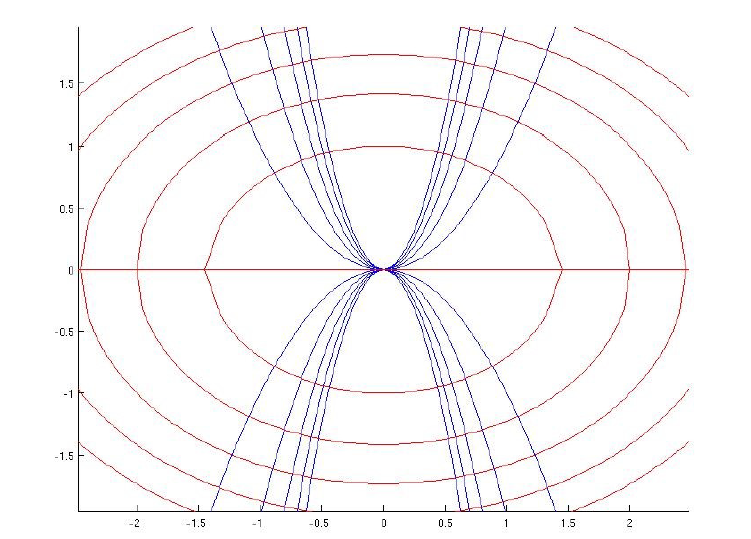
\includegraphics[width=0.65\linewidth]{Images/trayectortogonales.png}
    \caption{Familia de curvas y trayectorias ortogonales}
\end{figure}

\section{Métodos de integración de EDOs de primer orden}

\begin{theorem}{Th. de existencia y unicidad de solución}
    Sea la ED de primer orden $y^{\prime}=f(x,y)$ definida en un intervalo abierto $B$ del plano $P$ de $\mathbb{R}^2$ y si $f$ y $\frac{\partial f}{\partial y}$ son continuas en todo el abierto se verifica que:
    \begin{itemize}
        \item Para todo $(x_0,y_0)$ de $B$ existe una solución $g(x)$ definida en $(x_1,x_2)$ tal que $x_1<x_0<x_2$, que satisface la condición $g(x_0)=y_0$ (Existencia de solución).
        \item Si dos soluciones $y=g(x)$ e $y=h(x)$ coinciden en $x_0$ entonces las dos soluciones son idénticas en los puntos donde están definidas (Unicidad de solución).
    \end{itemize}
\end{theorem}

Si no exigimos que $\frac{\partial f}{\partial y}$ sea continua podemos garantizar que existe una solución pero no que sea única. A 
$(x_0,y_0)$ se le conocen como valores iniciales y a la relación $y_0=g(x_0)$ se le conoce como condición inicial.

\subsection{EDOs en variables separadas}

\subsubsection{$f(x,y)=f(x)$}

La solución general de la ED es una integral indefinida:

\begin{equation*}
    \frac{dy}{dx} = f(x) \Rightarrow \int \frac{dy}{dx} dx = \int f(x)\, dx \Rightarrow y = \int f(x) \, dx +c
\end{equation*}

\subsubsection{$f(x,y)=f(y)$}

Podemos encontrar la solución general integrando directamente:

\begin{equation*}
    \frac{dy}{dx} = f(y) \Rightarrow \int \frac{1}{f(y)}\frac{dy}{dx} dx = \int dx \Rightarrow \int \frac{dy}{f(y)} = x + c
\end{equation*}

Un ejemplo es la ley de desintegración radiactiva, $y^\prime=-ky$.

\subsubsection{$f(x,y)=f(x)g(y)$}

Podemos encontrar la solución separando las variables e integrando con respecto a cada una de las dos variables:

\begin{equation*}
    \frac{dy}{dx} = f(x)g(y) \Rightarrow \frac{1}{g(y)} \frac{dy}{dx} = f(x)dx \Rightarrow \int \frac{dy}{f(y)} = \int f(x)\,dx + c
\end{equation*}

\subsubsection{ED convertibles en variables separadas}

Son aquellas que mediante un cambio de variables pueden convertirse en ED de variables separadas, son de la forma:

\begin{equation*}
    \frac{dy}{dx} = f(ax + by) \quad a,b \in \mathbb{R}
\end{equation*}

Para resolverlas vamos a realizar el siguiente cambio de variable $x=ax + by$ para que $f$ dependa solo de $z$, una variable que depende de $x$, a continuación derivamos $z$:

\begin{equation*}
    \frac{dz}{dx} = a + b\frac{dy}{dx} = a +bf(z)
\end{equation*}

De esta forma obtenemos una ED cuya única variable dependiente es $z$ y cuya variable dependiente sigue siendo $x$:

\begin{equation*}
    \frac{dz}{dx}= a +bf(z) \Rightarrow \frac{dz}{a+bf(z)} = dx \Rightarrow \int \frac{dz}{a+bf(z)} = x + c 
\end{equation*}

Una vez calculada $z(x)$ deshacemos el cambio de variable para calcular la solución general $y(x)$:

\begin{equation*}
    y = \frac{z-ax}{b}
\end{equation*}

En caso de no poder despejar directamente $z(x)$ reemplazaríamos $z$ por $ax+by$.

\subsection{ED homogéneas}

Una función $f(x,y)$ es homogénea de grado n con respecto a $x$ e $y$ si verifica que:

\begin{equation*}
    f(tx,ty) = t^n f(x,y)
\end{equation*}

Algunos ejemplos son:

\begin{itemize}
    \item Homogénea de grado 1
    \begin{equation*}
        f(x,y)= \sqrt{x^2+y^2} \quad f(tx,ty) = \sqrt{(tx)^2+(ty)^2} = t f(x,y)
    \end{equation*}
    \item Homogénea de grado 0:
    \begin{equation*}
        f(x,y) = sen \left (\frac{x}{y}\right ) \quad f(tx,ty) = sen \left (\frac{tx}{ty}\right ) = t^0 sen \left (\frac{x}{y}\right )
    \end{equation*}
\end{itemize}

Además de eso podemos demostrar que una función homogénea de grado 0 con respecto a $x$ e $y$ se puede obtener como el cociente de dos funciones homogéneas del mismo grado:

\begin{equation*}
    f(tx,ty) = \frac{N(tx,ty)}{M(tx,ty)} = \frac{t^nN(x,y)}{t^nM(x,y)} = \frac{N(x,y)}{M(x,y)} = t^0 f(x,y)
\end{equation*}

Por tanto, podemos escribir cualquier función homogénea de grado 0 como función del cociente $y/x$, lo que nos ayudará a resolver ED homogéneas de grado 0:

\begin{equation*}
    f(tx,ty) = f(x,y) \forall t \Rightarrow \text{ Si } t=1/x \quad f(1,y/x) = f(x,y)
\end{equation*}

\par Si la ED es homogénea de grado 0 con respecto a $x$ e $y$ podemos resolverla con un cambio de variable dependiente para transformarla en una ED de variables separadas. El cambio que vamos a realizar es $y=zx$, que si derivamos con respecto a $x$ obtenemos:

\begin{equation*}
    y^{\prime} = z^{\prime}x+z
\end{equation*}

Por otra parte, podemos poner $f(x,y)$ como función del cociente $y/x$, por ser homogénea de grado 0, y aplicando el cambio de variable propuesto, también se puede escribir en función de $z$:

\begin{equation*}
    \begin{gathered}
    \frac{dz}{dx} = \frac{y^\prime - z}{x} = \frac{f(z)-z}{x} \Rightarrow \int \frac{dz}{f(z)-z} = \int \frac{dx}{x} \Rightarrow \ln |x| + c = \int \frac{dz}{f(z)-z} \\
    x = A \exp \left (\int \frac{dz}{f(z)-z}\right )
    \end{gathered}
\end{equation*}

Una vez determinada la solución general en las variables $z$ y $x$ hay que deshacer el cambio de variable para encontrar la solución $y$, para ello cambiamos $z$ por $y/x$

\subsubsection{ED convertibles en homogéneas}

Son de la forma:

\begin{equation*}
    \frac{dy}{dx} = f\left (\frac{ax + by +c}{\alpha x + \beta y + \gamma}\right ) \quad a,b,c,\alpha, \beta, \gamma \in \mathbb{R}
\end{equation*}

Podemos encontrarnos con dos situaciones:

\begin{itemize}
    \item Los coeficientes no son proporcionales, por lo que: 
    \begin{equation*}
        \begin{vmatrix}
            a & b \\
            \alpha & \beta
        \end{vmatrix} \neq 0
    \end{equation*}
    En este caso realizamos un cambio de variable dependiente y otro de variable independiente:
    \begin{equation*}
        \begin{gathered}
            x = X + x_1 \\
            y = Y + y_1
        \end{gathered}
    \end{equation*}
    Donde $x_1$ y $y_1$ son las soluciones del sistema:
    \begin{equation*}
        \left\{\begin{array}{l}
            ax + by + c =0 \\
            \alpha x + \beta y + \gamma =0
        \end{array}\right.
    \end{equation*}

    Queremos escribir la ED original en función de $X$ e $Y$, por lo que vamos a emplear la regla de la cadena para realizar el cambio de variable:
    \begin{equation*}
        \frac{dy}{dx} = \frac{d(Y+y_1)}{dx} = \frac{dY}{dx} = \frac{dY}{dX} \frac{dX}{dx} = \frac{dY}{dX}
    \end{equation*}


    Si reescribimos la ED en función de las nuevas variables obtenemos:

    \begin{equation*}
        f\left (\frac{ax + by +c}{\alpha x + \beta y + \gamma}\right )  = f \left (\frac{a(X+x_1)+b(Y+y_1)+c}{\alpha(X+x_1)+\beta(Y+y_1)+\gamma}\right ) = f\left (\frac{aX+bY}{\alpha X + \beta Y}\right )
    \end{equation*}

    La función $f(X,Y)$ obtenida es homogénea de grado 0 con respecto a $X$ e $Y$, por tanto la ED obtenida es homogénea:

    \begin{equation*}
        \frac{dY}{dX} = f \left (\frac{aX+bY}{\alpha X + \beta Y}\right )
    \end{equation*}

    Para resolverla vamos a realizar el cambio de variable $z=Y/X$, para convertirla en una ED de variables separadas. Cuando obtengamos la solución general para $z$ y $x$ hay que deshacer el cambio de variable para encontrar la solución general para $x$ e $y$.

    \item Los coeficientes son proporcionales, por lo que:
    \begin{equation*}
        \begin{vmatrix}
            a & b \\
            \alpha & \beta
        \end{vmatrix} = 0
    \end{equation*}
    En este caso la resolución es más sencilla. Aprovechando que $\alpha = na$ y $\beta =nb$ escribimos la ED como:
    \begin{equation*}
        \frac{dy}{dx} = f\left (\frac{ax + by +c}{na x + nb y + \gamma}\right ) = f\left (\frac{ax + by +c}{n(a x + b y) + \gamma}\right )
    \end{equation*}
\end{itemize}

Esta es una ED convertible en variables separadas, mediante el cambio $z=ax+by$.

\newpage

\subsection{ED lineales}

Las ED lineales de primer orden son de la forma:

\begin{equation*}
    \frac{dy}{dx} + p(x)y = f(x)
\end{equation*}

Donde $p(x)$ y $f(x)$ son funciones continuas. Podemos distinguir dos tipos de ED lineales:

\subsubsection{ED lineales homogéneas}

Cuando $f(x)=0$, en este caso la ED es de variables separadas:

\begin{equation*}
    \begin{gathered}
    \frac{dy}{dx} = -p(x)y \Rightarrow \frac{dy}{y} = -p(x)dx \Rightarrow \ln y = -\int p(x)\,dx + c \\ y = A \exp -\left (\int p(x)\, dx\right )
    \end{gathered}
\end{equation*}

\subsubsection{ED lineales inhomogéneas}

Cuando $f(x)\neq 0$. En este caso para obtener la solución general vamos a aplicar el principio de superposición de soluciones:

\begin{enumerate}
    \item Resolvemos primero la homogénea asociada
    \begin{equation*}
        y_H = A \exp -\left (\int p(x)\, dx\right )
    \end{equation*}
    \item Construimos una función prueba similar, pero suponiendo que $A$ no es una constante, sino una función de $x$:
    \begin{equation*}
        y_P = A(x) \exp -\left (\int p(x)\, dx\right )
    \end{equation*}
    \item Sustituímos en la ED la función prueba y calculamos la función $A(x)$ que hace que $y_P$ sea una solución particular.
    \item La solución general es la combinación de las dos, la homogénea asociada y la particular:
    \begin{equation*}
        y = y_H + y_P
    \end{equation*}
\end{enumerate}

\newpage

\subsection{ED reducibles a ED lineales}

\subsubsection{Ecuación de Bernoulli}

Es una ED de la forma:

\begin{equation*}
    \frac{dy}{dx} + p(x)y = f(x)y^n \quad n\neq 1
\end{equation*}

También la podemos expresar, dividiendo entre $y^n$ ambos lados, de la siguiente forma:

\begin{equation*}
    y^{-n} \frac{dy}{dx} + p(x)y^{1-n} = f(x) \quad n\neq1
\end{equation*}

Para resolverla vamos a emplear el siguiente cambio de variable dependiente:

\begin{equation*}
    z = y^{1-n}
\end{equation*}

Teniendo en cuenta esa relación vamos a buscar también una relación entre sus derivadas:

\begin{equation*}
    \frac{dz}{dx} = (1-n)y^{-n}\frac{dy}{dx} \Rightarrow \frac{1}{1-n} \frac{dz}{dx} = y^{-n}\frac{dy}{dx}
\end{equation*}

Por tanto, la ED en $z$ queda de la forma:

\begin{equation*}
    \frac{1}{1-n} \frac{dz}{dx} + p(x)z = f(x) \quad n\neq 1
\end{equation*}

que es una ED lineal inhomogénea que podemos resolver.

\subsubsection{Ecuación de Ricatti}

Es una ED de la forma:

\begin{equation*}
    \frac{dy}{dx} + p(x)y + q(x)y^2 = f(x)
\end{equation*}

Para encontrar una solución general necesitamos conocer de antemano una solución particular cualquiera $y_1(x)$. Vamos a resolverla con el cambio de variable $y=y_1 + z$, que la convierte en una ED de Bernoulli en $z(x)$. 

\par En primer lugar vamos a determinar la relación entre $y^\prime$ y $z^\prime$:

\begin{equation*}
    \frac{dy}{dx} = \frac{dy_1}{dx} + \frac{dz}{dx} = y_1^{\prime} + z^\prime
\end{equation*}

Si sustituímos $y$ e $y\prime$ en la ecuación de Ricatti:

\begin{equation*}
    y_1{^\prime} + z^\prime + p(x)y_1 + p(x)z + q(x)y_1^2 + q(x)z^2 + 2q(x)y_1z=f(x)
\end{equation*}

Como $y_1$ es solución de la ecuación de Ricatti tenemos que:

\begin{equation*}
    y_1^{\prime} +p(x)y_1 + q(x)y_1^2 = f(x)
\end{equation*}

Por tanto la ED queda de la forma:

\begin{equation*}
    z^\prime + p(x)z + q(x)z^2 + 2q(x)y_1z = 0
\end{equation*}

Obtenemos así una ED de Bernoulli con $n=2$ que podemos resolver.

\subsection{ED exactas}

Sea una ED de la forma:

\begin{equation*}
    M(x,y)dx+ N(x,y)dy=0
\end{equation*}

Si existe una función $f(x,y)$ tal que:

\begin{equation*}
    \frac{\partial f}{\partial x} = M(x,y) \quad \text{y} \quad \frac{\partial f}{\partial y} = N(x,y)
\end{equation*}

Entonces podemos reescribir la ED como:

\begin{equation*}
    df = \frac{\partial f}{\partial x}dx + \frac{\partial f}{\partial y} dy =0
\end{equation*}

Por lo que la solución general será de la forma: $f(x,y)=C$. Si esto se verifica diremos que la ED es exacta. Para comprobar que una ED es exacta debemos verificar la siguiente condición, que es condición necesaria y suficiente:

\begin{equation*}
    \frac{\partial M}{\partial y} = \frac{\partial N}{\partial x}
\end{equation*}

Además de eso $M$, $N$ y sus derivadas parciales tienen que ser continuas.

\par Para resolver ED exactas vamos a emplear el método de integración:

\newpage

\begin{enumerate}
    \item En primer lugar, dado que $M(x,y)=\frac{\partial f}{\partial x}$, integrando esta expresión respecto a x obtenemos la función $f(x,y)$, salvo una función desconocida $g(y)$.
    \item Si ahora derivamos esta expresión respecto a $y$ deberíamos obtener $N(x,y)$:
    \begin{equation*}
        \frac{\partial f}{\partial y} = \frac{\partial}{\partial y} \left (\int M(x,y)\,dx\right ) + \frac{\partial g(y)}{\partial y} = N(x,y)
    \end{equation*}
    \item Si despejamos $g(y)$ y integramos respecto aa $y$ podemos calcular el valor de $g(y)$ y, por tanto, de $f(x,y)$:
    \begin{equation*}
        \begin{gathered}
        g(y) = \int \left [N(x,y)- \frac{\partial}{\partial y}\left (\int M(x,y)\,dx \right )\right ]\,dy \\
        f(x,y) = \int M(x,y)\, dx + \int \left [N(x,y)- \frac{\partial}{\partial y}\left (\int M(x,y)\,dx \right )\right ]\,dy = C
        \end{gathered}
    \end{equation*}
\end{enumerate}

\subsection{Factores integrantes}

Si la ED $M(x,y)dx+ N(x,y)dy=0$ no es exacta pero existe una función $\mu(x,y)$ tal que la ED $\mu(x,y)\left (M(x,y)dx+ N(x,y)dy\right )=0$ es exacta, entonces denominamos a la función $\mu(x,y)$ un factor integrante de la ED. Toda ecuación diferencial con solución tiene algún factor integrante. La condición que debe verificar $\mu(x,y)$ para ser un factor integrante es:

\begin{equation*}
    \begin{gathered}
    \frac{\partial (\mu M(x,y))}{\partial y} = \frac{\partial (\mu N(x,y))}{\partial x} \Rightarrow \frac{\partial \mu}{\partial y} + \mu \frac{\partial M}{\partial y} = \frac{\partial \mu}{\partial x} N +\mu \frac{\partial N}{\partial x} \\
    \frac{1}{\mu} \left (\frac{\partial \mu}{\partial y}M-\frac{\partial \mu}{\partial x}N\right ) = \frac{\partial N}{\partial x} - \frac{\partial M}{\partial y}
    \end{gathered}
\end{equation*}

Esta es una ED en derivadas parciales, difícil de resolver, pero que en casos concretos podemos resolver de forma más sencilla para calcular un factor integrante:

\subsubsection{$\mu = \mu(x)$}

En este caso la parcial con respecto a $y$ se anula y obtenemos la siguiente ED:

\begin{equation*}
    \frac{1}{\mu} \left (\frac{\partial \mu}{\partial x}N \right ) =\frac{\partial N}{\partial x} - \frac{\partial M}{\partial y}
\end{equation*}

Esta ED ya no tiene derivadas parciales, por lo que podemos resolverla para encontrar un factor integrante $\mu(x)$ pasando el diferencial al otro lado e integrando en ambos miembros:

\begin{equation*}
    \begin{gathered}
    \frac{d\mu}{\mu} = \frac{1}{N} \left (\frac{\partial N}{\partial x} - \frac{\partial M}{\partial y}\right ) dx \\
    \mu = \exp \left (\frac{1}{N} \left (\frac{\partial N}{\partial x} - \frac{\partial M}{\partial y}\right ) dx \right )
    \end{gathered}
\end{equation*}

Los factores integrantes son cualesquiera de las soluciones particulares de la ED, por eso no es necesario añadir la constante.

\subsubsection{$\mu = \mu(y)$}

En este caso la parcial con respecto a $x$ se anula y obtenemos la siguiente ED:

\begin{equation*}
    \frac{1}{\mu} \left (-\frac{\partial \mu}{\partial y}M \right ) =\frac{\partial N}{\partial x} - \frac{\partial M}{\partial y}
\end{equation*}

El procedimiento es idéntico al anterior:

\begin{equation*}
    \begin{gathered}
        \frac{d\mu}{\mu} = \frac{1}{M} \left (\frac{\partial M}{\partial y} - \frac{\partial N}{\partial x} \right ) dy \\
        \mu = \exp \left (\frac{1}{N} \left (\frac{\partial M}{\partial y} - \frac{\partial N}{\partial x} \right ) dy \right )
    \end{gathered}
\end{equation*}

\section{Reducción de orden}

En ocasiones, mediante un cambio de variable, podemos reducir el orden de una ED para resolverla de forma más sencilla:

\subsection{$F(x,y^{\prime k},y^{\prime k+1},...,y^n)=0$}

En los casos en los que en la ED no aparece $y$ ni sus derivadas de orden menor que $k$ podemos hacer el cambio de variable dependiente $z=y^{\prime k}$ para obtener una ED de orden $n-k$. Un ejemplo sería la ED:

\begin{equation*}
    y^{\prime \prime \prime} + y^{\prime \prime }=0 \overbrace{\Rightarrow}^{z=y^{\prime \prime}} z^\prime +z =0
\end{equation*}

\subsection{La ED no contiene $x$}

Si la ED no tiene variable independiente se puede reducir el orden en una unidad haciendo el cambio de variable $y^{\prime}=p$, considerando a $y$ como la nueva variable independiente. Las derivadas sucesivas se calculan aplicando la regla de la cadena:

\begin{equation*}
    \begin{gathered}
        y^\prime = \frac{dy}{dx} = p(y) \\
        y^{\prime \prime} = \frac{dp(y)}{dx} = \frac{dp}{dy} \frac{dy}{dx} = p \frac{dp}{dy} \\
        y^{\prime \prime \prime} = \frac{d}{dx}\left (p\frac{dp}{dy}\right ) = \frac{d}{dy} \left (p\frac{dp}{dy}\right ) \frac{dy}{dx} = \left (\frac{dp}{dy}\frac{dp}{dy} + p \frac{d^2p}{dy}\right )p = p(p^\prime)^2+p^2p^{\prime \prime}
    \end{gathered}
\end{equation*}

\subsection{ED homogénea de grado $n$}

Si la ED es homogénea de grado $n$ respecto a $y$ y sus sucesivas derivadas podemos hacer el siguiente cambio de variable dependiente:

\begin{equation*}
    y = e^{\int z \,dx}
\end{equation*}

Donde $z$ es una función desconocida que depende de $x$. Para reducir el orden calculamos las sucesivas derivadas del cambio de variable y las sustituimos en la ED:

\begin{equation*}
    \begin{gathered}
        y^\prime = z \exp \int z \, dx \\
        y^{\prime \prime} = z^{\prime} \exp \int z\,dx + z^2 \exp \int z\,dx
    \end{gathered}
\end{equation*}

Teniendo en cuenta el carácter homogéneo de la ED con respecto a $y$ y sus derivadas se podrá sacar la exponencial como factor común, de forma que obtenemos una ED de $z$ de orden $n-1$.

\newpage

\subsection{Derivada de otra función}

Si el primer miembro de la ED $F(x,y,y^\prime,...,y^{\prime n})=0$ es la derivada de una cierta función $G(x,y,y^\prime,...,y^{\prime n-1})$:

\begin{equation*}
    F(x,y,y^\prime,...,y^{\prime n})=\frac{d}{dx}G(x,y,y^\prime,...,y^{\prime n-1})
\end{equation*}

Un ejemplo es la ED $yy^{\prime \prime} + (y^{\prime})^2=1$:

\begin{equation*}
    \begin{gathered}
    \left (yy^\prime\right )^\prime = 1\\
    yy^\prime = x + c \\
    \int y \,dy = \int (x+c)\, dx \\
    \frac{y^2}{2} = \frac{x^2}{2} + cx + d
    \end{gathered}
\end{equation*}



\end{document}